\documentclass[11pt,a4paper]{article}
\usepackage[margin=2.5cm]{geometry}
\usepackage{amsmath,amssymb}
\usepackage{graphicx}
\usepackage{xcolor}
\usepackage{booktabs}
\usepackage{microtype}
\usepackage[numbers,sort&compress]{natbib}
\usepackage[colorlinks=true,linkcolor=blue!50!black,citecolor=blue!50!black,urlcolor=blue!50!black]{hyperref}
\usepackage{caption}
\hypersetup{pdftitle={Conditioning of periapsis-shift extraction from orbit integrations: an accumulated-phase estimator and its error scaling},pdfauthor={Uppala Sri Sai Vithesh},pdfsubject={Numerical conditioning of periapsis-shift extraction in Schwarzschild orbit integrations}}
\captionsetup{font=small,labelfont=bf}
\setlength{\parskip}{0.4em}
\setlength{\parindent}{0pt}
\emergencystretch=3em
\newcommand{\PooledWins}{69}
\newcommand{\PooledTotal}{80}
\newcommand{\PooledMedianRatio}{11.2}
\newcommand{\WinsRK}{38}
\newcommand{\NRK}{40}
\newcommand{\MedRatioRK}{6.8}
\newcommand{\WinsDop}{31}
\newcommand{\NDop}{40}
\newcommand{\MedRatioDop}{13.4}
\newcommand{\NLoss}{11}
\newcommand{\LossShiftMin}{4.4}
\newcommand{\GridShiftMin}{$2.4\times10^{-5}$}
\newcommand{\GridShiftMax}{49}
\newcommand{\EventFloor}{$7.5\times10^{-13}$}
\newcommand{\ModelCorrect}{69}
\newcommand{\ModelTotal}{80}
\newcommand{\RhoMedianA}{0.77}
\newcommand{\RhoNA}{30}
\newcommand{\RhoQlowA}{0.09}
\newcommand{\RhoQhighA}{3.4}
\newcommand{\RhoMedianB}{0.78}
\newcommand{\RhoNB}{40}
\newcommand{\LossRhoList}{0.8, 0.95, 0.99}
\newcommand{\CubicValid}{36}
\newcommand{\CubicRuns}{288}
\newcommand{\CubicRefCheck}{$1.7\times10^{-70}$}
\newcommand{\CubicWinsMin}{35}
\newcommand{\CubicOf}{36}
\newcommand{\CubicMedLow}{21}
\newcommand{\CubicMedHigh}{60}
\newcommand{\CubicShiftMin}{$8.6\times10^{-4}$}
\newcommand{\CubicShiftMax}{1.7}
\newcommand{\CubicPhaseMaxErr}{$9.4\times10^{-13}$}
\newcommand{\MercNaiveEllipk}{$1.9\times10^{-9}$}
\newcommand{\MercNaiveQuad}{$9.3\times10^{-11}$}
\newcommand{\MercStableQuad}{$1.9\times10^{-16}$}
\newcommand{\MaxNaiveEllipk}{$1.9\times10^{-11}$}
\newcommand{\MaxNaiveQuad}{$6.6\times10^{-11}$}
\newcommand{\MaxStableQuad}{$5.9\times10^{-16}$}
\newcommand{\MercDopEvent}{$1.8\times10^{-6}$}
\newcommand{\MercDopPhase}{$5.1\times10^{-13}$}
\newcommand{\MercShift}{$5.0\times10^{-7}$}
\newcommand{\MercArcsecRef}{42.9807}
\newcommand{\MercArcsecEvent}{42.980770}
\newcommand{\MercArcsecPhase}{42.980694}
\newcommand{\MercEventSixMin}{1.13}
\newcommand{\MercEventSixMax}{2.34}
\newcommand{\DriftMin}{$2.5\times10^{-15}$}
\newcommand{\DriftMax}{$2.0\times10^{-13}$}
\newcommand{\PeakParaMax}{$4.0\times10^{-9}$}
\newcommand{\PeakRawMax}{$3.1\times10^{-3}$}
\newcommand{\RefCheckMax}{$3.0\times10^{-71}$}
\newcommand{\MercDrift}{$2.9\times10^{-15}$}
\newcommand{\MercRho}{$1.7\times10^{-7}$}
\newcommand{\MercRhoInv}{$5.9\times10^{6}$}
\newcommand{\MercRatioMin}{$1.1\times10^{6}$}
\newcommand{\MercRatioMax}{$4.5\times10^{7}$}
\newcommand{\MercEps}{$2.7\times10^{-8}$}
\newcommand{\MercE}{0.2056}
\newcommand{\PyVer}{3.12.3}
\newcommand{\NumpyVer}{2.5.4}
\newcommand{\ScipyVer}{1.18.1}
\newcommand{\MpDps}{70}
\newcommand{\SameWins}{59}
\newcommand{\SameOf}{80}
\newcommand{\SameMedRatio}{2.3}
\newcommand{\SameWinsRK}{35}
\newcommand{\SameWinsDop}{24}
\newcommand{\SameLossRho}{0.2, 0.5, 0.8, 0.95, 0.99}
\newcommand{\SameWorstRatio}{$8.9\times10^{-3}$}
\newcommand{\SensMedPA}{0.80}
\newcommand{\SensDomFrac}{54}
\newcommand{\AugSmallerPct}{91}
\newcommand{\AugMedFactor}{2.1}
\newcommand{\EndLowWins}{30}
\newcommand{\EndLowN}{30}
\newcommand{\EndLowMed}{$3.9\times10^{3}$}
\newcommand{\SameLowWins}{30}
\newcommand{\SameLowMed}{$1.3\times10^{3}$}
\newcommand{\SameMidWins}{16}
\newcommand{\SameMidN}{20}
\newcommand{\SameMidMed}{1.8}
\newcommand{\SameHighWins}{13}
\newcommand{\SameHighN}{30}
\newcommand{\SameHighMed}{0.98}
\newcommand{\EndHighWins}{19}
\newcommand{\EndHighN}{30}
\newcommand{\LsodaWinsMin}{15}
\newcommand{\LsodaWinsMax}{18}
\newcommand{\LsodaMedRatio}{0.90}
\newcommand{\StrongRatioTopRho}{1.000}
\newcommand{\SmallEPhaseAtMin}{$7.8\times10^{-13}$}
\newcommand{\SmallEPhaseAtRef}{$2.1\times10^{-14}$}
\newcommand{\SmallEEventAtMin}{$2.0\times10^{-11}$}
\newcommand{\CubicSameWins}{141}
\newcommand{\CubicSameN}{144}
\newcommand{\CubicSameMed}{12.3}
\newcommand{\CubicRhoMin}{$2.6\times10^{-4}$}
\newcommand{\CubicRhoMax}{0.47}
\newcommand{\CubicPA}{0.64}
\newcommand{\RootChangeMax}{34}
\newcommand{\RootRuns}{16}
\newcommand{\HPmaxEvent}{$6.7\times10^{-31}$}
\newcommand{\HPmaxPhase}{$6.6\times10^{-31}$}
\newcommand{\HPmaxW}{$6.0\times10^{-33}$}
\newcommand{\HPmaxPsi}{$7.7\times10^{-33}$}
\newcommand{\HPn}{7}
\newcommand{\HPmaxSec}{3}
\newcommand{\OrderRaw}{1.00}
\newcommand{\OrderExactMin}{3.00}
\newcommand{\OrderExactMax}{3.00}
\newcommand{\FloorMerc}{$3.8\times10^{-12}$}
\newcommand{\FloorHigh}{$2.3\times10^{-10}$}
\newcommand{\ExactFineMax}{$1.3\times10^{-13}$}
\newcommand{\ScAugCtlSmallerPct}{91}
\newcommand{\ScAugFreeSmallerPct}{20}
\newcommand{\ScMedPlainOverCtl}{2.1}
\newcommand{\ScNfevCtl}{1.08}
\newcommand{\ScNfevFree}{0.96}
\newcommand{\ScCostReached}{69}
\newcommand{\ScN}{80}
\newcommand{\ObsWinsAll}{45}
\newcommand{\ObsMedAll}{1.05}
\newcommand{\CmWinsAll}{46}
\newcommand{\CmMedAll}{1.9}
\newcommand{\ObsLowWins}{30}
\newcommand{\ObsLowMed}{307}
\newcommand{\CmLowWins}{30}
\newcommand{\CmLowMed}{$1.6\times10^{3}$}
\newcommand{\CtlLowWins}{30}
\newcommand{\CtlLowMed}{$1.3\times10^{3}$}
\newcommand{\EteLowWins}{30}
\newcommand{\EteLowMed}{$3.1\times10^{3}$}
\newcommand{\ScLowN}{30}
\newcommand{\ObsMidWins}{8}
\newcommand{\ObsMidMed}{0.922}
\newcommand{\CmMidWins}{10}
\newcommand{\CmMidMed}{0.964}
\newcommand{\CtlMidWins}{16}
\newcommand{\CtlMidMed}{1.75}
\newcommand{\EteMidWins}{20}
\newcommand{\EteMidMed}{4.37}
\newcommand{\ScMidN}{20}
\newcommand{\ObsHighWins}{7}
\newcommand{\ObsHighMed}{0.398}
\newcommand{\CmHighWins}{6}
\newcommand{\CmHighMed}{0.667}
\newcommand{\CtlHighWins}{13}
\newcommand{\CtlHighMed}{0.978}
\newcommand{\EteHighWins}{20}
\newcommand{\EteHighMed}{1.16}
\newcommand{\ScHighN}{30}


\newcommand{\dphi}{\Delta\varphi}

\title{Conditioning of periapsis-shift extraction from orbit integrations:\\
an accumulated-phase estimator and its error scaling}
\author{Uppala Sri Sai Vithesh\thanks{Corresponding author: \href{mailto:srisaivitheshuppala99@gmail.com}{srisaivitheshuppala99@gmail.com}}\\
\small Independent Student Researcher, Andhra Pradesh, India}
\date{22 November 2026}

\begin{document}
\maketitle

\begin{abstract}
Numerical orbit integrations often give the relativistic periapsis shift as the azimuth of the next periapsis minus $2\pi$, a difference of order-one numbers whose error does not shrink with the shift. We examine this conditioning problem for bound timelike geodesics of the Schwarzschild spacetime and evaluate the shift instead by integrating the phase deviation $\psi=\theta-\varphi$ of the orbit in the $(w-1,-w')$ plane, whose rate is $O(\varepsilon)$ and known in closed form. At periapsis the rate equals $-\rho$, where $\rho=\varepsilon(6+2e)<1$ measures proximity to the separatrix (more generally $-\delta(1+e)/e$ for a perturbation $\delta$), so the contribution from event-time error is reduced by the factor $\rho$. Against a 70-digit reference, independently confirmed by a 35-digit Taylor-series integration, the phase estimator run as a separate integration was more accurate in \PooledWins{} of \PooledTotal{} comparisons (\texttt{RK45} and \texttt{DOP853}, $\mathrm{rtol}=10^{-12}$, median error ratio \PooledMedianRatio). Beyond $\rho\approx0.05$ most of that advantage is not due to the observable: appending $\psi$ to the state makes it a strict step-size controller. With $\psi$ excluded from the error control the gain is about \ObsLowMed{} for $\rho\le0.05$, absent for $0.05<\rho\le0.5$ and reversed for $\rho>0.5$; at equal cost the estimator is better only for $\rho\le0.05$ (median ratio \CmLowMed). The effect is solver dependent and absent with \texttt{LSODA}. A cancellation-free quadrature is more accurate than every ODE-based estimator tested, so the method concerns only cases where the shift must be extracted from an integration, and in practice weak-field orbits such as Mercury's. A cubic-perturbation model with an independent reference shows a gain on a common trajectory (\CubicSameWins{} of \CubicSameN{} runs, $\rho_{\rm gen}\le\CubicRhoMax$). The paper introduces no new gravitational physics; code and data are supplied.
\end{abstract}

\section{Introduction}

The advance of the periapsis of a bound orbit is a classic relativistic effect. In the Schwarzschild spacetime the shift per radial period is known in closed form through elliptic integrals \citep{Hall2008}. Analytic treatments exist for other spacetimes, for example Kerr and Kerr--de~Sitter \citep{Kraniotis2006}, and Katsumata et al.\ \citep{Katsumata2025} derived series representations without special functions for Kerr and Chazy--Curzon, building on an exact Schwarzschild series by Walters \citep{Walters2018}, and noted their use for checking numerical integrations. For any static spherically symmetric metric the shift reduces to a one-dimensional quadrature.

Numerical orbit tools nevertheless integrate the equations of motion directly. PyGRO is a Python integrator for general-relativistic orbits \citep{DellaMonica2025}, and Li et al.\ \citep{Li2026} describe a Mathematica/OpenMP framework for rational orbits and gravitational waveforms in static spherically symmetric spacetimes. We have not examined how these codes extract the periapsis shift, and nothing in this paper is a criticism of them. The numerical issue considered here is more general. If the shift is obtained as the azimuth $\varphi_{\rm peri}$ of the next periapsis minus $2\pi$, it is a small difference between two numbers of order one. The accuracy of the event azimuth depends on the global trajectory error, event localisation, dense-output interpolation \citep{Shampine1991,Shampine2000}, and rounding. These error sources need not decrease with the size of the shift. The relative error of the shift therefore grows as the shift decreases, the familiar cancellation problem of floating-point arithmetic \citep{Higham2002}. For Mercury the shift per orbit is of order $10^{-7}$~rad.

A phase-plane representation of an orbit by an amplitude and an intrinsic phase has been used by Pantig and \"Ovg\"un \citep{PantigOvgun2026} for the weak deflection of light: the bending angle follows from the excess azimuth accumulated while the intrinsic phase advances between fixed asymptotic endpoints, and an all-order series in $M/b$ is obtained analytically. The two approaches share the idea of extracting an observable from accumulated excess azimuth. The present work addresses a different problem: bound timelike orbits, numerical integration of a phase deviation, and the conditioning of the resulting periapsis-shift estimate.

\textbf{Contributions.} This work develops: (i)~an accumulated-phase estimator for the periapsis shift, with an exact local sensitivity $\psi'_{\rm peri}=-\rho$ (generalised to $-\delta(1+e)/e$). (ii)~a comparison with event subtraction against an independently checked reference, using four protocols (end-to-end, same trajectory, observable only and cost-matched) that separate the effect of the observable from the effect of step-size control. (iii)~an assessment of the regimes where the estimator helps, is neutral, or performs worse, including strong-field and small-eccentricity cases and four solvers; (iv)~comparisons with double-precision closed-form and cancellation-free quadrature baselines; (v)~tests on a cubic-perturbation family with an independent quadrature reference; and (vi)~an analysis of the order of accuracy of three-point peak interpolation. \textbf{Scope.} The paper introduces no new gravitational physics, does not claim that integrating a small deviation instead of differencing large numbers is a new idea, and tests no Kerr, non-planar, dissipative or time-dependent system. The literature search was not systematic, so no priority claim is made.

\section{Orbit model and reference values}

We use $G=c=M=1$. Equatorial bound timelike geodesics are parametrised by $w=p/r$, with periapsis and apoapsis at $w=1+e$ and $w=1-e$, semi-latus rectum $p$ and eccentricity $e$, and $\varepsilon=M/p$. As a function of the azimuth $\varphi$,
\begin{equation}
w''+w = k+3\varepsilon w^{2},\qquad k=1-\varepsilon(3+e^{2}),
\label{eq:orbit}
\end{equation}
where primes denote $d/d\varphi$ and $k$ is fixed by requiring $w=1\pm e$ to be turning points (Appendix~\ref{app:deriv}). The quantity $J=\tfrac12 w'^2+\tfrac12 w^2-kw-\varepsilon w^3$ is conserved. Bound orbits require
\begin{equation}
\rho\equiv\varepsilon(6+2e)<1,
\label{eq:rho}
\end{equation}
and $\rho\to1$ is the separatrix. The first integral factorises as $w'^2=(1+e-w)(w-1+e)\,Q(w)$ with $Q(w)=1-4\varepsilon-2\varepsilon w$, so with $w=1+e\cos\chi$ the azimuth advanced per radial period is
\begin{equation}
\Phi=\int_0^{2\pi}\frac{d\chi}{\sqrt{1-(6+2e\cos\chi)\varepsilon}}
=\frac{4}{\sqrt{1-2(3-e)\varepsilon}}\,K\!\left(\frac{4e\varepsilon}{1-2(3-e)\varepsilon}\right),
\label{eq:exact}
\end{equation}
with $K(m)$ the complete elliptic integral of the first kind in terms of the parameter $m$. The periapsis shift is $\dphi=\Phi-2\pi$, with the weak-field expansion $\dphi=6\pi\varepsilon+\tfrac{3\pi}{2}(18+e^2)\varepsilon^2+O(\varepsilon^3)$. Note $Q(1+e)=1-\rho$.

All algebraic identities of this section and of Sec.~\ref{sec:est} were verified symbolically (32 SymPy checks, supplied as a script). The reference $\dphi$ is computed with \texttt{mpmath} at \MpDps{} digits from the exact binary value of the double-precision $(\varepsilon,e)$ used by the integrators; the elliptic and direct-quadrature forms agree to \RefCheckMax{} or better. It is independently confirmed by a 35-digit Taylor-series ODE integration that shares no algebra with Eq.~\eqref{eq:exact} (Sec.~\ref{sec:hp}).

\textbf{Grid.} $e\in\{0.01,0.1,0.3,0.6,0.9\}$ and $\rho\in\{10^{-5},10^{-3},0.05,0.2,0.5,0.8,0.95,0.99\}$ give 40 configurations with exact shifts from \GridShiftMin{} to \GridShiftMax{}~rad per radial period. \textbf{Mercury.} $GM_\odot=1.32712440018\times10^{20}$~m$^3$\,s$^{-2}$ \citep{Montenbruck2000}, semi-major axis $5.790905\times10^{10}$~m, $e=0.20563069$ and period $87.9691$~d \citep{NASAMercury} give $\varepsilon=$~\MercEps, $\rho=$~\MercRho{} and a shift of \MercArcsecRef{} arcsec per century from Eq.~\eqref{eq:exact}. This is the Schwarzschild test-particle contribution only. The observed perihelion advance of Mercury is dominated by classical effects (planetary perturbations and the precession of the reference frame), and general relativity contributes about $43''$ per century; none of the classical effects is modelled here.

\section{Estimators}
\label{sec:est}

\subsection{Event subtraction}
Starting at periapsis ($\varphi=0$, $w=1+e$, $w'=0$), integrate Eq.~\eqref{eq:orbit} to the next downward crossing of $w'=0$ at $\varphi_{\rm ev}$ and set $\dphi_{\rm event}=\varphi_{\rm ev}-2\pi$. Its error is exactly the error $\delta\varphi_{\rm ev}=\varphi_{\rm ev}-\Phi$ of the event azimuth. This error has several distinct sources: the global trajectory error accumulated by the solver, the root localisation within the step, the interpolation error of the dense output, and rounding. Their relative sizes depend on the solver; we make no a-priori claim that $\delta\varphi_{\rm ev}$ equals the requested tolerance times $\varphi_{\rm ev}$, and Sec.~\ref{sec:hp} measures one of them (root localisation) separately.

\subsection{Accumulated phase}
Let $X=(w-1)/e$ and $Y=-w'/e$, and $\theta=\operatorname{atan2}(Y,X)$, so $\theta=0$ at periapsis. Then
\begin{equation}
\theta'=\frac{XY'-YX'}{X^2+Y^2}=\frac{w'^2-(w-1)\,w''}{(w-1)^2+w'^2}.
\end{equation}
Write Eq.~\eqref{eq:orbit} as $w''=-(w-1)+\delta(w)$ with $\delta(w)=\varepsilon(3w^2-3-e^2)$. The deviation $\psi\equiv\theta-\varphi$ obeys
\begin{equation}
\psi'=-\frac{(w-1)\,\delta(w)}{(w-1)^2+w'^2}
=-\varepsilon\,\frac{(w-1)(3w^2-3-e^2)}{(w-1)^2+w'^2},
\label{eq:psi}
\end{equation}
which is exact algebra, so the nearly unit quantity $\theta'$ is never formed and subtracted from 1. We integrate $\psi$ with $(w,w')$ from $\psi(0)=0$ and set $\dphi_{\rm phase}=-\psi(\varphi_{\rm ev})$. This is correct because $\theta(\varphi_{\rm ev})=2\pi$: $w'$ vanishes only at the two turning points ($Q>0$), $X$ decreases monotonically from $1$ to $-1$ on the first half-cycle while $Y>0$, and the curve never reaches the origin, so $\theta$ advances by exactly $\pi$ on each half-cycle; hence $\psi(\varphi_{\rm ev})=2\pi-\varphi_{\rm ev}=-\dphi$. No phase unwrapping is needed because $\psi'$ rather than $\theta$ is integrated.

\subsection{Properties}
\textbf{(i) Size.} $\psi'=O(\varepsilon)$ and is integrated directly.
\textbf{(ii) Event-time sensitivity.} At periapsis $w=1+e$, $w'=0$, so $\delta=e\rho$ and
\begin{equation}
\psi'_{\rm peri}=-\rho\quad\text{exactly.}
\label{eq:sens}
\end{equation}
Because $w$ is even about periapsis, $\psi'$ is even too, so an event-time error $\delta\varphi_{\rm ev}$ changes $\dphi_{\rm phase}$ by $\rho\,\delta\varphi_{\rm ev}+O(\delta\varphi_{\rm ev}^3)$ while it changes $\dphi_{\rm event}$ by $\delta\varphi_{\rm ev}$. This is a statement about the \emph{local sensitivity to the event time only}. It does not say that the full error ratio equals $1/\rho$, because the phase estimator also accumulates its own integration error in $\psi$ (Sec.~\ref{sec:decomp}).
\textbf{(iii) Regularity.} $(w-1)^2+w'^2=e^2\left[\cos^2\chi+\sin^2\chi\,Q(1+e\cos\chi)\right]\ge e^2(1-\rho)$, so Eq.~\eqref{eq:psi} is non-singular for $e>0$ and $\rho<1$. As $e\to0$, $\psi'$ has the finite limit $-6\varepsilon\cos^2\chi/[\cos^2\chi+\sin^2\chi(1-6\varepsilon)]$, but evaluating it from the state variables involves $w-1=e\cos\chi$, so rounding in $w$ is amplified by $1/e$ (Sec.~\ref{sec:strong}).
\textbf{(iv) Generalisation.} For any autonomous equation $w''=-(w-1)+\delta(w)$ the identity $\psi'=-(w-1)\delta(w)/[(w-1)^2+w'^2]$ holds and the local sensitivity is $-\psi'_{\rm peri}=\delta(1+e)/e$. This is established algebraically. It has been tested numerically only for Eq.~\eqref{eq:orbit} and the cubic family of Sec.~\ref{sec:cubic}, not for any system that is not of this planar, autonomous form.

\subsection{Protocols and setup}
\label{sec:setup}
We use SciPy's \texttt{solve\_ivp} \citep{Virtanen2020} with \texttt{RK45} (Dormand--Prince 5(4) \citep{Dormand1980}), \texttt{DOP853} (Dormand--Prince 8(5,3) \citep{Hairer1993}), and, in Sec.~\ref{sec:solvers}, \texttt{LSODA} and \texttt{Radau}, with $\mathrm{rtol}\in\{10^{-6},\dots,10^{-13}\}$ and $\mathrm{atol}=10^{-16}$ (Mercury: also $10^{-12}$ to $10^{-18}$). The integration is split at $\varphi=\pi$ to exclude the initial periapsis from the event search. Four protocols are used. \emph{End-to-end}: the event estimator uses a plain integration of $(w,w')$ and the phase estimator a separate integration of $(w,w',\psi)$ whose error control includes $\psi$ (with $\mathrm{atol}=10^{-16}$ this makes $\psi$ a strict controller, because it is small). \emph{Same trajectory ($\psi$ in control)}: both estimators are evaluated on one integration of $(w,w',\psi)$ and one event time. \emph{Observable only}: the same, but with $\psi$ excluded from the error control (a huge \texttt{atol} on that component), so the trajectory is not controlled more tightly than in a plain run and the two estimators differ only in the observable. \emph{Cost-matched}: the event estimator comes from a plain run whose \texttt{rtol} is tightened by factors of $0.8$ until it uses at least as many right-hand-side evaluations as the augmented run (SciPy clamps \texttt{rtol} at $2.2\times10^{-14}$, so this was reached in \ScCostReached{} of \ScN{} runs). Errors are $|\dphi_{\rm num}-\dphi_{\rm ref}|$ (absolute) and that divided by $\dphi_{\rm ref}$ (relative).

\section{Results}

\subsection{Mercury-like orbit}
Table~\ref{tab:mercury} and Fig.~\ref{fig:mercury} show the end-to-end comparison. At $\mathrm{rtol}=10^{-6}$ the event estimator returns a shift wrong by \MercEventSixMin--\MercEventSixMax{} times its own size, i.e.\ no usable value, whereas the phase estimator is correct to a few $10^{-8}$--$10^{-7}$. The event/phase error ratio ranges from \MercRatioMin{} to \MercRatioMax{}, within an order of magnitude of $1/\rho=$~\MercRhoInv. At $\mathrm{rtol}=10^{-12}$ with \texttt{DOP853} the precession is \MercArcsecEvent{} (event) and \MercArcsecPhase{} (phase) arcsec per century against \MercArcsecRef{}. The numbers of right-hand-side evaluations agree to within about ten per cent.

\begin{table}[!htbp]
\centering
\caption{Mercury-like orbit ($\varepsilon=2.66\times10^{-8}$, $e=0.2056$; exact shift $\Delta\varphi=$~\MercShift~rad per radial period). Relative error of the extracted shift for the event and accumulated-phase estimators, with $\mathrm{atol}=10^{-16}$. The last column gives right-hand-side evaluations (event / phase).}
\label{tab:mercury}
\begin{tabular}{llcccc}
\toprule
Solver & rtol & event & phase & event/phase & nfev \\
\midrule
DOP853 & $10^{-6}$ & 1.13 & $2.6\times10^{-7}$ & $4.3\times10^{6}$ & 319 / 295 \\
DOP853 & $10^{-8}$ & 0.0377 & $1.2\times10^{-9}$ & $3.3\times10^{7}$ & 343 / 379 \\
DOP853 & $10^{-10}$ & $2.5\times10^{-4}$ & $3.2\times10^{-11}$ & $7.8\times10^{6}$ & 403 / 415 \\
DOP853 & $10^{-12}$ & $1.8\times10^{-6}$ & $5.1\times10^{-13}$ & $3.5\times10^{6}$ & 535 / 523 \\
DOP853 & $10^{-13}$ & $1.4\times10^{-7}$ & $7.3\times10^{-14}$ & $1.9\times10^{6}$ & 607 / 607 \\
RK45 & $10^{-6}$ & 2.34 & $5.3\times10^{-8}$ & $4.5\times10^{7}$ & 298 / 292 \\
RK45 & $10^{-8}$ & 0.0114 & $3.6\times10^{-10}$ & $3.2\times10^{7}$ & 472 / 496 \\
RK45 & $10^{-10}$ & $4.4\times10^{-5}$ & $2.5\times10^{-11}$ & $1.8\times10^{6}$ & 1060 / 1042 \\
RK45 & $10^{-12}$ & $1.6\times10^{-7}$ & $1.5\times10^{-13}$ & $1.1\times10^{6}$ & 2566 / 2464 \\
RK45 & $10^{-13}$ & $1.2\times10^{-8}$ & $9.1\times10^{-15}$ & $1.4\times10^{6}$ & 4000 / 3844 \\
\bottomrule
\end{tabular}
\end{table}


\begin{figure}[!htbp]
\centering
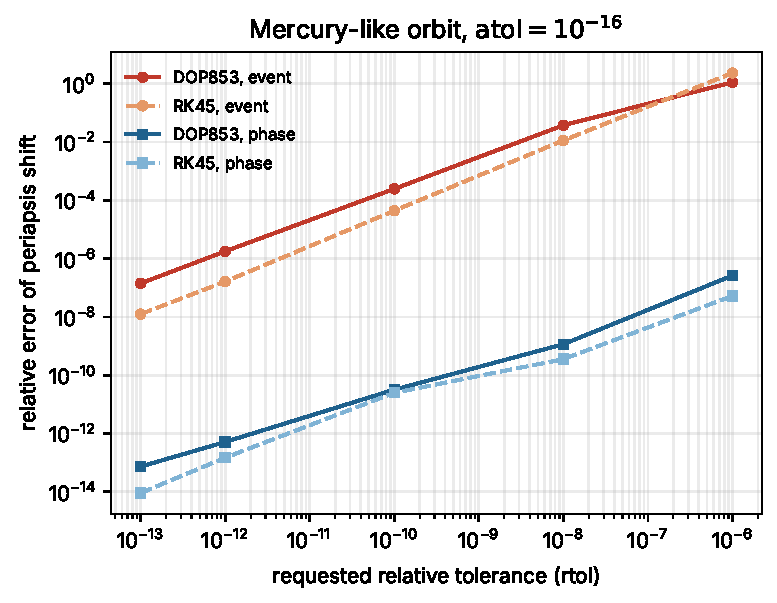
\includegraphics[width=0.62\textwidth]{figures/fig01_mercury_tolerance.pdf}
\caption{Relative error of the extracted Mercury-like shift versus requested tolerance, end-to-end protocol.}
\label{fig:mercury}
\end{figure}

\subsection{Schwarzschild grid: four protocols}
\label{sec:grid}
\textbf{End-to-end} at $\mathrm{rtol}=10^{-12}$ the phase estimator has the smaller error in \WinsRK{} of \NRK{} cases for \texttt{RK45} (median ratio \MedRatioRK) and \WinsDop{} of \NDop{} for \texttt{DOP853} (median \MedRatioDop), \PooledWins{} of \PooledTotal{} pooled (Appendix Table~\ref{tab:winrate} gives other tolerances); all \NLoss{} losses occur at $\rho\in\{\LossRhoList\}$. These numbers come from the original grid code. Re-running the end-to-end comparison with a differently coded but algebraically identical right-hand side gives the same event errors to better than one per cent but phase errors that differ case by case by factors of up to about five, because the phase estimator's error at small $\rho$ is close to the rounding level; we therefore interpret medians and bins, not individual ratios (Table~\ref{tab:protocol}: its end-to-end column uses the second coding and shows \EteHighWins{} wins for $\rho>0.5$, against \EndHighWins{} of \EndHighN{} in the original grid).

\textbf{Is the end-to-end advantage due to the observable?} Largely not, beyond small $\rho$. Appending $\psi$ to the state and keeping it in the error control makes the event error smaller than in a plain run in \ScAugCtlSmallerPct\% of the \ScN{} runs, by a median factor of \ScMedPlainOverCtl{}, at \ScNfevCtl{} times the evaluations. If $\psi$ is excluded from the error control, the event error is smaller than in the plain run in only \ScAugFreeSmallerPct\% of runs, at \ScNfevFree{} times the cost. Table~\ref{tab:protocol} then shows what the observable alone achieves. For $\rho\le0.05$ the phase estimator wins in all \ScLowN{} runs under every protocol, with a median ratio of \ObsLowMed{} (observable only) to \EteLowMed{} (end-to-end). For $0.05<\rho\le0.5$ the advantage rests on the step control: observable only it wins \ObsMidWins{} of \ScMidN{} (median \ObsMidMed), cost-matched \CmMidWins{} of \ScMidN{} (\CmMidMed). For $\rho>0.5$ it is worse: \ObsHighWins{} of \ScHighN{} wins (median \ObsHighMed{}) observable only and \CmHighWins{} of \ScHighN{} (\CmHighMed) at equal cost. Pooled over all 80 runs the observable-only comparison gives \ObsWinsAll{} wins (median \ObsMedAll) and the cost-matched one \CmWinsAll{} (median \CmMedAll), the latter dominated by small $\rho$. With $\psi$ in the control the pooled same-trajectory count is \SameWins{} of \SameOf{} (median \SameMedRatio; \texttt{RK45} \SameWinsRK{}/40, \texttt{DOP853} \SameWinsDop{}/40), with losses at $\rho\in\{\SameLossRho\}$ and a worst-case ratio of \SameWorstRatio. Using $\psi$ as a strict controller is a real effect of the augmented formulation, but it is equivalent to a slightly tighter tolerance and is not a property of the phase observable.

\begin{table}[!htbp]
\centering
\caption{Four comparison protocols at $\mathrm{rtol}=10^{-12}$ (80 runs: 40 configurations, \texttt{RK45} and \texttt{DOP853}), grouped by $\rho$; each cell gives phase wins and the median ratio of event error to phase error. \emph{End-to-end}: event estimator from a plain integration, phase estimator from a separate integration with $\psi$ appended to the state and included in the error control. \emph{$\psi$ in control}: both estimators from the one augmented trajectory. \emph{Observable only}: as before, but $\psi$ excluded from the error control (huge \texttt{atol} on that component), so the trajectory is not better controlled than in the plain run. \emph{Cost-matched}: event estimator from a plain run whose tolerance is tightened until it uses at least as many right-hand-side evaluations as the augmented run, against the phase estimator of that run.}
\label{tab:protocol}
\small
\begin{tabular}{lcccccccc}
\toprule
 & \multicolumn{2}{c}{end-to-end} & \multicolumn{2}{c}{$\psi$ in control} & \multicolumn{2}{c}{observable only} & \multicolumn{2}{c}{cost-matched} \\
 & wins & ratio & wins & ratio & wins & ratio & wins & ratio \\
\midrule
$\rho\le0.05$ & 30 / 30 & $3.1\times10^{3}$ & 30 / 30 & $1.3\times10^{3}$ & 30 / 30 & 307 & 30 / 30 & $1.6\times10^{3}$ \\
$0.05<\rho\le0.5$ & 20 / 20 & 4.37 & 16 / 20 & 1.75 & 8 / 20 & 0.922 & 10 / 20 & 0.964 \\
$\rho>0.5$ & 20 / 30 & 1.16 & 13 / 30 & 0.978 & 7 / 30 & 0.398 & 6 / 30 & 0.667 \\
\bottomrule
\end{tabular}
\end{table}


\subsection{Where the phase error comes from}
\label{sec:decomp}
On a single trajectory (here with $\psi$ in the control, but the algebra does not depend on this) the phase error can be decomposed. Linearising about the exact event, $\dphi_{\rm phase}-\dphi_{\rm ref}=\rho_{\rm loc}\,\delta\varphi_{\rm ev}-\eta$, where $\rho_{\rm loc}=-\psi'$ evaluated at the numerical event state and $\eta$ collects the accumulated error of $\psi$, including the propagated trajectory error. Both $\delta\varphi_{\rm ev}$ and the left-hand side are measured against the exact reference, so $\eta$ is obtained by difference. Fig.~\ref{fig:same}, left, plots the actual phase error against $\rho_{\rm loc}\delta\varphi_{\rm ev}$: the points follow the diagonal over ten decades. The median ratio of predicted to actual error is \SensMedPA{}, but the event-time term exceeds $|\eta|$ in only \SensDomFrac\% of runs. The statement ``phase error $\approx\rho\times$ event error'' is therefore a description of the typical case, not a bound. Fig.~\ref{fig:same}, right, shows that the event/phase error ratio tracks $1/\rho$ for $\rho\le0.05$ and then scatters below it, down to the worst case quoted above. An empirical description of the end-to-end absolute errors as a roughly constant floor for the event estimator and an error roughly proportional to $\dphi$ for the phase estimator is given in Appendix~\ref{app:tables}; it is phenomenological and does not predict individual winners.

\begin{figure}[!htbp]
\centering
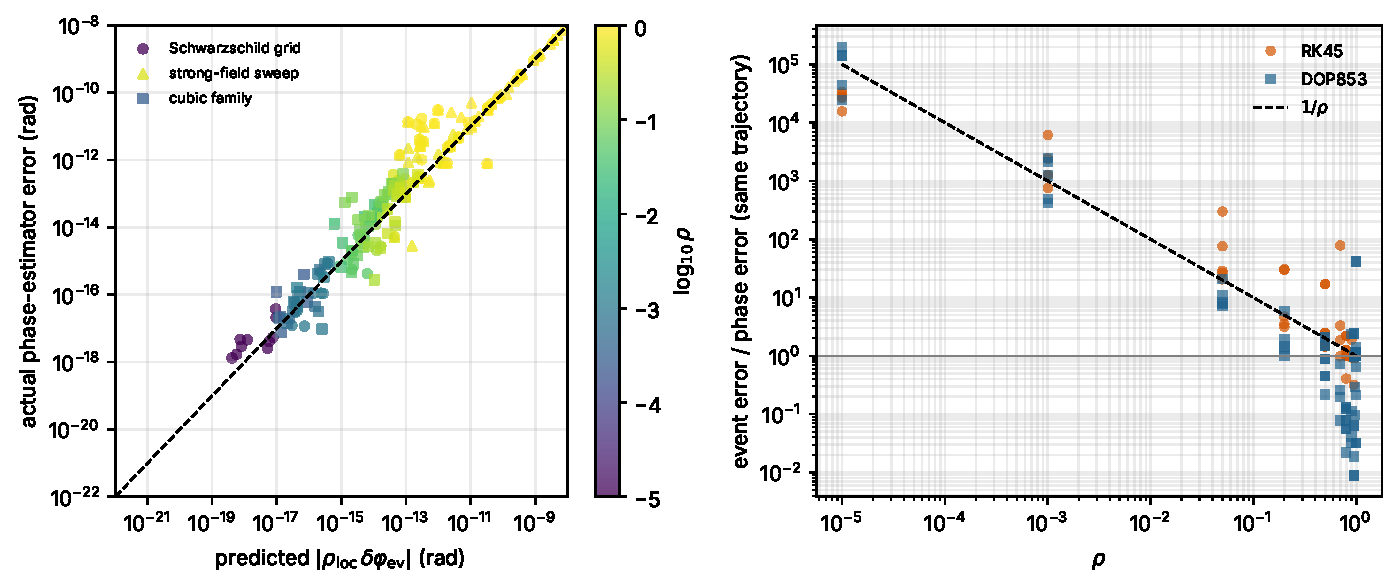
\includegraphics[width=\textwidth]{figures/fig02_same_trajectory.pdf}
\caption{Same-trajectory protocol, $\mathrm{rtol}=10^{-12}$. Left: actual phase-estimator error against the predicted event-time contribution $|\rho_{\rm loc}\delta\varphi_{\rm ev}|$ (dashed: equality; colour: $\log_{10}\rho$; Schwarzschild grid, strong-field sweep and cubic family). Right: event error over phase error against $\rho$ (dashed: $1/\rho$).}
\label{fig:same}
\end{figure}

\subsection{Solver dependence}
\label{sec:solvers}
Table~\ref{tab:solvers} (Appendix) repeats the same-trajectory comparison with \texttt{LSODA} and \texttt{Radau}. The benefit is solver dependent. \texttt{Radau} and \texttt{RK45} behave similarly, \texttt{DOP853} shows a smaller advantage, and \texttt{LSODA} shows none (phase wins \LsodaWinsMin--\LsodaWinsMax{} of 40, median ratio about \LsodaMedRatio). We have not investigated the cause. All solvers are from one library, so we cannot say how far this generalises to other implementations.

\subsection{Strong field and small eccentricity}
\label{sec:strong}
Table~\ref{tab:strong} samples $\rho$ up to 0.999. As $\rho\to1$ the sensitivity factor tends to unity, so the two estimators converge (median ratio \StrongRatioTopRho{} at $\rho=0.999$). In the intermediate range the accumulated error of $\psi$ exceeds the event-time term (median $|\eta|/|\rho\,\delta\varphi_{\rm ev}|$ of 2 to 4 at $\rho=0.7$ and $0.8$) and the phase estimator is worse in the median at those values. For small eccentricity (Appendix Table~\ref{tab:smalle}) the phase estimator still wins in 5 of 6 cases at every tested $e$ down to $10^{-4}$, but its median relative error rises from \SmallEPhaseAtRef{} at $e=0.01$ to \SmallEPhaseAtMin{} at $e=10^{-4}$, consistent with the $1/e$ amplification of rounding noted in Sec.~\ref{sec:est}. The event estimator degrades too (\SmallEEventAtMin{} at $e=10^{-4}$).

\begin{table}[!htbp]
\centering
\caption{Strong-field sweep (same-trajectory protocol with $\psi$ in the error control, $\mathrm{rtol}=10^{-12}$, $e\in\{0.1,0.3,0.6,0.9\}$, both solvers). $\eta$ is the part of the phase error not explained by the event-time term (Sec.~\ref{sec:decomp}).}
\label{tab:strong}
\begin{tabular}{ccccc}
\toprule
$\rho$ & median shift (rad) & phase wins & median ratio & median $|\eta|/|\rho\,\delta\varphi_{\rm ev}|$ \\
\midrule
0.5 & 2.1 & 6 / 8 & 1.52 & 0.38 \\
0.7 & 3.9 & 3 / 8 & 0.86 & 2 \\
0.8 & 5.4 & 4 / 8 & 0.57 & 4.4 \\
0.9 & 8.2 & 4 / 8 & 0.98 & 0.47 \\
0.95 & 11.1 & 3 / 8 & 0.98 & 0.11 \\
0.98 & 14.9 & 4 / 8 & 0.99 & 0.07 \\
0.99 & 17.8 & 6 / 8 & 1.00 & 0.02 \\
0.995 & 20.7 & 6 / 8 & 1.00 & 0.0057 \\
0.999 & 27.3 & 7 / 8 & 1.00 & 0.001 \\
\bottomrule
\end{tabular}
\end{table}


\subsection{Comparison with closed forms and quadrature}
A user who can evaluate Eq.~\eqref{eq:exact} in double precision faces the same subtraction of $2\pi$ (Fig.~\ref{fig:baselines}, Table~\ref{tab:baselines}). For Mercury the double-precision $K(m)$ form has relative error \MercNaiveEllipk{} and a plain quadrature \MercNaiveQuad. Both are better than the ODE event estimator at every tolerance tested and worse than the ODE phase estimator at $\mathrm{rtol}\le10^{-10}$. A quadrature of the cancellation-free integrand $(1-s)^{-1/2}-1=s/[\sqrt{1-s}(1+\sqrt{1-s})]$ with $s=(6+2e\cos\chi)\varepsilon$, which removes the subtraction analytically, reaches \MercStableQuad{} for Mercury and at worst \MaxStableQuad{} over the grid, better than every ODE-based result. The reference is built from the exact binary $\varepsilon$ that the solvers use; building it from the decimal representation instead changes these quadrature errors by up to a factor of five, which is why we state the convention.

\begin{table}[!htbp]
\centering
\caption{Relative error of the periapsis shift over the 40-configuration grid (ODE rows: rtol $=10^{-12}$, $\mathrm{atol}=10^{-16}$) against the 70-digit reference.}
\label{tab:baselines}
\begin{tabular}{lcc}
\toprule
Method & median & maximum \\
\midrule
ODE, DOP853, event extractor & $1.9\times10^{-12}$ & $4.0\times10^{-8}$ \\
ODE, DOP853, phase extractor & $2.9\times10^{-13}$ & $2.5\times10^{-12}$ \\
closed form $K(m)$, double precision, subtract $2\pi$ & $1.2\times10^{-15}$ & $1.9\times10^{-11}$ \\
quadrature, double precision, subtract $2\pi$ & $8.4\times10^{-16}$ & $6.6\times10^{-11}$ \\
quadrature, cancellation-free integrand & $7.6\times10^{-17}$ & $5.9\times10^{-16}$ \\
\bottomrule
\end{tabular}
\end{table}


\begin{figure}[!htbp]
\centering
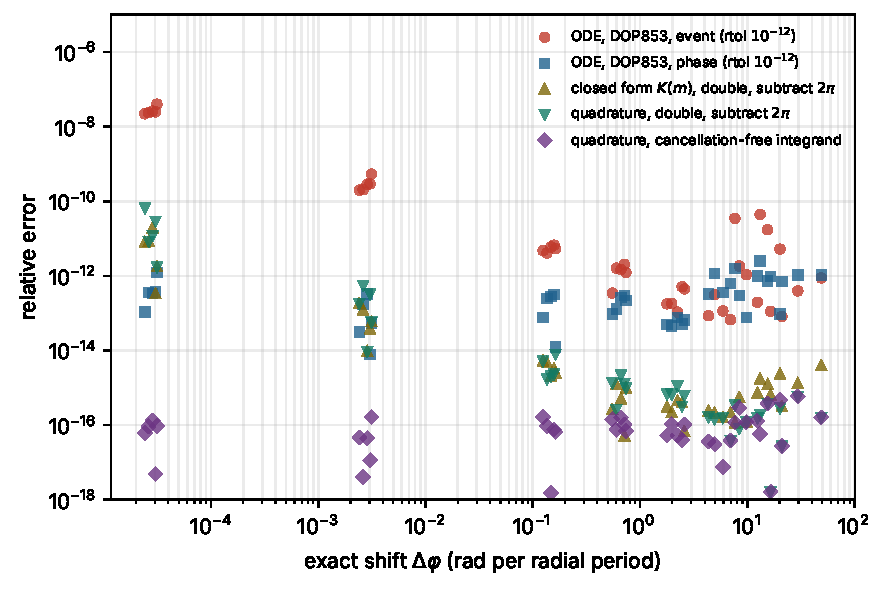
\includegraphics[width=0.72\textwidth]{figures/fig03_baselines.pdf}
\caption{Relative error over the 40-configuration grid: ODE estimators (\texttt{DOP853}, $\mathrm{rtol}=10^{-12}$, end-to-end) and double-precision closed-form and quadrature baselines against the 70-digit reference.}
\label{fig:baselines}
\end{figure}

\subsection{A force law without the Schwarzschild closed form}
\label{sec:cubic}
To test that the behaviour is not tied to the Schwarzschild force law we add a cubic term, $w''+w=k+3\varepsilon w^2+\gamma w^3$ with $k=1-\varepsilon(3+e^2)-\gamma(1+e^2)$, again chosen so that $1\pm e$ are turning points. This is a model, not a specific spacetime. The first integral factorises exactly, $w'^2=(1+e-w)(w-1+e)\,Q(w)$ with
\begin{equation}
Q(w)=-\tfrac{\gamma}{2}w^2-(2\varepsilon+\gamma)w+1-2(2\varepsilon+\gamma)+\tfrac{\gamma}{2}(1-e^2),
\end{equation}
so that $\Phi=\int_0^{2\pi}d\chi/\sqrt{Q(1+e\cos\chi)}$, which reduces to Eq.~\eqref{eq:exact} at $\gamma=0$ and supplies a reference independent of the elliptic form. Since $w''(1+e)=-eQ(1+e)$ and $w''(1-e)=+eQ(1-e)$, the orbit is a genuine bound orbit with real azimuth, no further turning points and a regular integrand exactly when $Q>0$ on $[1-e,1+e]$ (a quadratic, so endpoints and, if inside, the vertex suffice). The phase rate is Eq.~\eqref{eq:psi} with $\delta(w)=-\varepsilon(3+e^2)-\gamma(1+e^2)+3\varepsilon w^2+\gamma w^3$ and the local sensitivity is $\rho_{\rm gen}=\delta(1+e)/e=1-Q(1+e)$. We take $\varepsilon\in\{10^{-4},10^{-2},0.04\}$, $e\in\{0.1,0.3,0.6\}$ and $\gamma/\varepsilon\in\{\pm0.3,\pm1\}$, all \CubicValid{} of which are admissible (shifts \CubicShiftMin{} to \CubicShiftMax{} rad), with both solvers and $\mathrm{rtol}\in\{10^{-10},10^{-12}\}$ (\CubicRuns{} end-to-end runs). Table~\ref{tab:cubic} shows that the phase estimator wins in at least \CubicWinsMin{} of \CubicOf{} configurations in every setting. On a single trajectory it wins \CubicSameWins{} of \CubicSameN{} runs (median ratio \CubicSameMed), and the predicted-to-actual error ratio has median \CubicPA{} with $\rho_{\rm gen}$ ranging from \CubicRhoMin{} to \CubicRhoMax{}. The shifts stay at or below about 1.7~rad, so the test does not reach the strong-field regime.

\begin{table}[!htbp]
\centering
\caption{Cubic-perturbation family: phase-accumulator wins out of 36 configurations, and the median and minimum event/phase relative-error ratio.}
\label{tab:cubic}
\begin{tabular}{llccc}
\toprule
Solver & rtol & phase wins & median ratio & minimum ratio \\
\midrule
RK45 & $10^{-10}$ & 35 / 36 & 44.0 & 0.89 \\
DOP853 & $10^{-10}$ & 36 / 36 & 49.7 & 1.88 \\
RK45 & $10^{-12}$ & 35 / 36 & 60.0 & 0.35 \\
DOP853 & $10^{-12}$ & 35 / 36 & 21.1 & 0.72 \\
\bottomrule
\end{tabular}
\end{table}


\begin{figure}[!htbp]
\centering
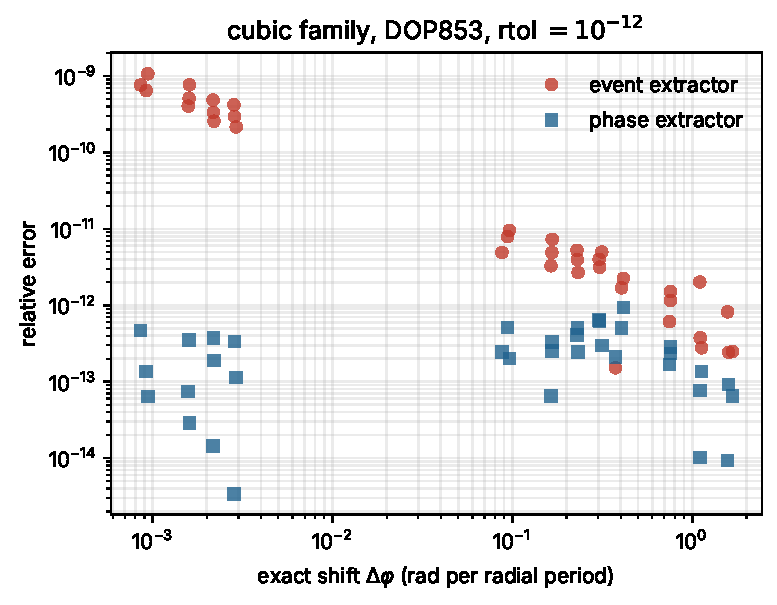
\includegraphics[width=0.52\textwidth]{figures/fig04_cubic_family.pdf}
\caption{Cubic-perturbation family, end-to-end: relative error of the two estimators against the exact shift (\texttt{DOP853}, $\mathrm{rtol}=10^{-12}$).}
\label{fig:cubic}
\end{figure}

\subsection{Independent reference and event-root tests}
\label{sec:hp}
A Taylor-series ODE integration at 35 digits (\texttt{mpmath.odefun}, tolerance $10^{-28}$) was run for \HPn{} cases (including a small-$e$ and a cubic case; each took at most \HPmaxSec{}~s). It shares no algebra with the quadrature reference. At the quadrature's $\Phi$, $|w'|\le$~\HPmaxW{} and $|\psi+\dphi|\le$~\HPmaxPsi{}; the event azimuth and the phase estimate in this arithmetic agree with the quadrature to \HPmaxEvent{} and \HPmaxPhase{} respectively (Appendix Table~\ref{tab:hp}). This confirms the reference, the winding argument and the sign convention, and shows that event subtraction itself is unproblematic in extended precision, so the conditioning problem belongs to double precision with a finite tolerance.

To isolate root localisation, we solved with dense output and located the root of $w'$ by Brent's method with tolerance from $10^{-4}$ to $10^{-16}$, independently of the ODE tolerance (\RootRuns{} solver/tolerance/case combinations). The event error changes by at most \RootChangeMax\% over twelve decades of root tolerance. At $\mathrm{rtol}$ of $10^{-8}$ and $10^{-12}$ the event error is therefore not limited by root finding on the dense output but by the trajectory itself.

\subsection{Locating periapsis from samples}
Table~\ref{tab:interp} and Fig.~\ref{fig:interp} show the maximum azimuth error of a periapsis located from samples on a uniform grid of $N$ points per $2\pi$, now measured against the exact periapsis angle. The raw sampled maximum converges with observed order \OrderRaw{} (error $\le h/2$). The three-point parabolic vertex converges with observed order \OrderExactMin{} (identical to two decimals for all three orbits and every $N$) when the samples are exact, not the second order that is usual for generic peaks. This is expected here: $w$ is even about periapsis, so the leading $h^2$ term of the vertex error vanishes and the remaining error is proportional to the offset of the peak from the grid, which is itself $O(h)$. With samples rounded to double precision, or taken from a double-precision ODE solution, the error stops improving between $N\approx3000$ and $10^4$. It plateaus at about \FloorMerc{} for the Mercury-like orbit at $N=31623$ and, for the strongest field ($\varepsilon=0.15$), grows with $N$ to \FloorHigh{}: the vertex formula divides small differences of nearly equal samples, so rounding in the samples is amplified by up to about $1/h$. An earlier version of this experiment measured the error against a numerically located event time and sampled with $\mathrm{atol}=10^{-14}$; its plateau mixed these effects and is not reproduced here.

\begin{table}[!htbp]
\centering
\caption{Peak (periapsis) location from samples on a uniform grid of $N$ points per $2\pi$: maximum azimuth error over 20 grid offsets against the \emph{exact} periapsis angle. ``Exact'' samples are 35-digit values from the Taylor-series ODE solution; ``rounded'' are the same samples rounded to double precision; ``ODE'' samples come from a double-precision \texttt{DOP853} dense output ($\mathrm{rtol}=10^{-13}$, $\mathrm{atol}=10^{-16}$). Parabolic = three-point vertex.}
\label{tab:interp}
\small
\begin{tabular}{lccccc}
\toprule
Orbit & $N$ & raw maximum & parabolic, exact & parabolic, rounded & parabolic, ODE \\
\midrule
Mercury-like & 100 & 0.0314 & $4.0\times10^{-6}$ & $4.0\times10^{-6}$ & $4.0\times10^{-6}$ \\
Mercury-like & 1000 & $3.1\times10^{-3}$ & $4.0\times10^{-9}$ & $4.0\times10^{-9}$ & $4.0\times10^{-9}$ \\
Mercury-like & 10000 & $3.1\times10^{-4}$ & $4.0\times10^{-12}$ & $4.6\times10^{-12}$ & $6.0\times10^{-12}$ \\
Mercury-like & 31623 & $9.9\times10^{-5}$ & $1.3\times10^{-13}$ & $3.8\times10^{-12}$ & $4.9\times10^{-12}$ \\
$\varepsilon=0.05,\ e=0.3$ & 100 & 0.0305 & $2.4\times10^{-6}$ & $2.4\times10^{-6}$ & $2.4\times10^{-6}$ \\
$\varepsilon=0.05,\ e=0.3$ & 1000 & $3.1\times10^{-3}$ & $2.4\times10^{-9}$ & $2.4\times10^{-9}$ & $2.4\times10^{-9}$ \\
$\varepsilon=0.05,\ e=0.3$ & 10000 & $3.1\times10^{-4}$ & $2.4\times10^{-12}$ & $3.4\times10^{-12}$ & $8.8\times10^{-12}$ \\
$\varepsilon=0.05,\ e=0.3$ & 31623 & $9.8\times10^{-5}$ & $7.7\times10^{-14}$ & $3.8\times10^{-12}$ & $8.2\times10^{-12}$ \\
$\varepsilon=0.15,\ e=0.3$ & 100 & 0.0309 & $6.8\times10^{-7}$ & $6.8\times10^{-7}$ & $6.8\times10^{-7}$ \\
$\varepsilon=0.15,\ e=0.3$ & 1000 & $3.1\times10^{-3}$ & $6.8\times10^{-10}$ & $6.8\times10^{-10}$ & $6.8\times10^{-10}$ \\
$\varepsilon=0.15,\ e=0.3$ & 10000 & $3.1\times10^{-4}$ & $6.8\times10^{-13}$ & $6.0\times10^{-11}$ & $1.2\times10^{-10}$ \\
$\varepsilon=0.15,\ e=0.3$ & 31623 & $9.9\times10^{-5}$ & $2.1\times10^{-14}$ & $2.3\times10^{-10}$ & $2.5\times10^{-10}$ \\
\bottomrule
\end{tabular}
\end{table}


\begin{figure}[!htbp]
\centering
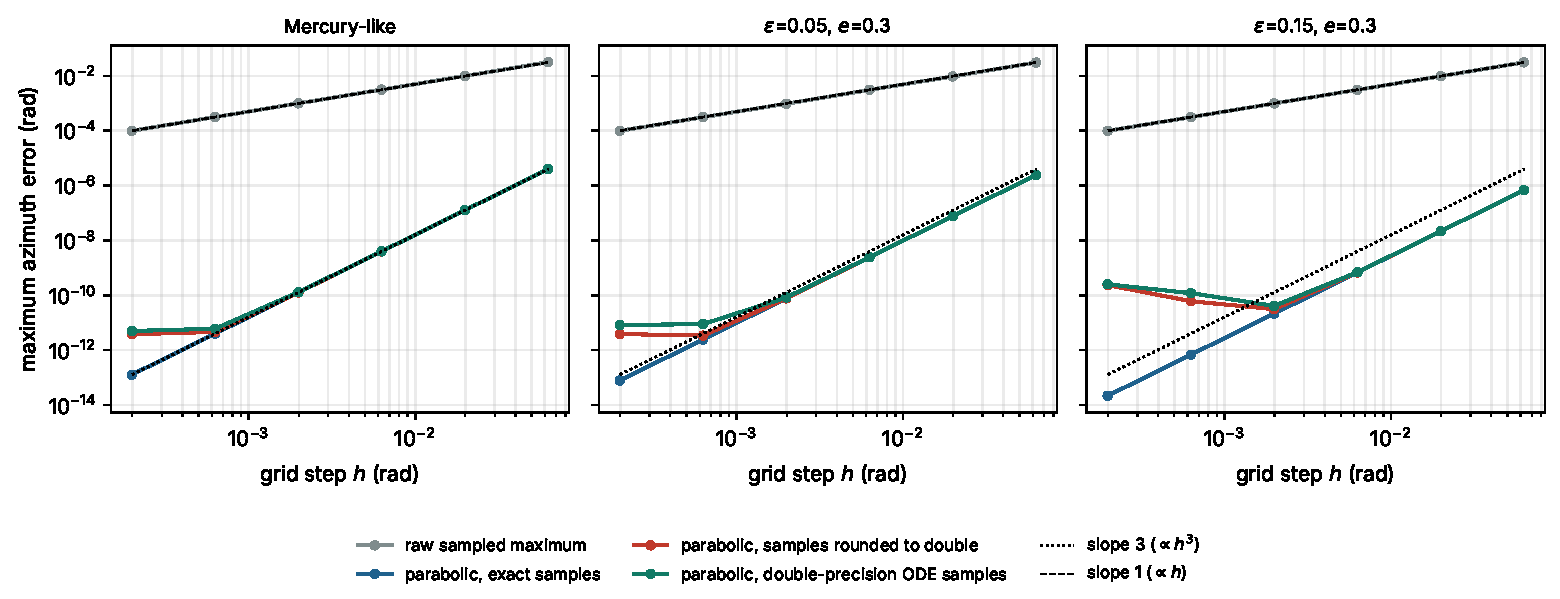
\includegraphics[width=\textwidth]{figures/fig05_interpolation_convergence.pdf}
\caption{Maximum periapsis-azimuth error versus grid step for the raw sampled maximum and the parabolic vertex, with exact, double-rounded and double-precision-ODE samples. Dotted: slope~3; dashed: slope~1.}
\label{fig:interp}
\end{figure}

\subsection{When should each extraction method be used?}
\label{sec:use}
\begin{itemize}
\item \textbf{Cancellation-free quadrature} whenever the shift can be written as a one-dimensional integral, which is the case for every static spherically symmetric metric and for the cubic family: it was the most accurate method tested (relative error at most \MaxStableQuad{} on the grid).
\item \textbf{Accumulated phase} when the shift must come from an orbit integration and $\rho\lesssim0.05$, that is weak-field orbits such as Mercury-like ones: it won in every run under every protocol, with a gain of order $1/\rho$ (median \ObsLowMed{} observable only, \CmLowMed{} cost-matched). It needs a reference centre and scale ($w=1$, $e$), which presuppose a roughly elliptic orbit. Including $\psi$ in the error control also lowered the event time error by a median factor of \ScMedPlainOverCtl{} at about \ScNfevCtl{} times the cost.
\item \textbf{Event subtraction} is adequate for $\rho\gtrsim0.05$: at equal cost the phase estimator was neutral for $0.05<\rho\le0.5$ and worse above, and the shift is then of order one so that its relative error is of the order of the trajectory error. It is also unproblematic in extended precision.
\item \textbf{The phase estimator is poorly conditioned} for $e\to0$ (rounding amplified by $1/e$; usable to $10^{-4}$ here), for $\rho\gtrsim0.5$ where the accumulated error of $\psi$ can dominate and it was up to about a hundred times worse than event subtraction in the worst case, and with solvers such as \texttt{LSODA} where we observed no benefit.
\end{itemize}

\section{Discussion and limitations}

\textbf{Scope.} The accumulated phase removes the cancellation, and Eq.~\eqref{eq:sens} explains the size of the gain at small $\rho$, where it is robust. It is not a general improvement. The headline end-to-end count of \PooledWins{} of \PooledTotal{} overstates the effect of the observable: with $\psi$ excluded from the error control it is \ObsWinsAll{} of \ScN{}, and at equal cost \CmWinsAll{} of \ScN{}, concentrated at $\rho\le0.05$. Closed-form or quadrature evaluation with a stable integrand is more accurate wherever it applies. The practical niche is therefore weak-field orbits integrated numerically, and possibly integrations that carry additional dynamics (extra forces, spin or tidal terms, dissipation, N-body perturbations) for which no quadrature exists. These are possible applications; \emph{none was tested}, and the algebraic generalisation of Sec.~\ref{sec:est} is verified numerically only for the two autonomous planar families above. We did not test whether the observable-only and cost-matched conclusions at $\rho>0.05$ also hold for the cubic family.

\textbf{What we tested.} Planar orbits; four solvers from one library in double precision (the explicit RK pair, \texttt{DOP853}, \texttt{LSODA}, \texttt{Radau}); SciPy's event detection; one model deviation beyond Schwarzschild with shifts up to 1.7~rad; no Kerr or non-planar orbits, no symplectic integrators, no dissipative or time-dependent forces. The empirical fits in Appendix Table~\ref{tab:fits} have low $R^2$ for the event estimator and predict the winner in \ModelCorrect{} of \ModelTotal{} cases, no better than always predicting a phase win. Strong-field losses are described qualitatively through the decomposition of Sec.~\ref{sec:decomp} rather than explained quantitatively, and the solver dependence is unexplained.

\textbf{Related work.} See the Introduction. In brief: exact and series formulae for the periapsis shift \citep{Hall2008,Kraniotis2006,Katsumata2025} supply references and checks and are preferable where available; PyGRO and the framework of Li et al.\ \citep{DellaMonica2025,Li2026} are numerical orbit tools whose handling of the shift we have not examined; the phase-plane formulation of Pantig and \"Ovg\"un \citep{PantigOvgun2026} is an analytic treatment of light deflection and a different problem.

\section{Reproducibility}
\label{sec:repro}
All tables, figures and numbers quoted through macros are generated from the CSV files by the scripts of the accompanying archive (\texttt{research\_analysis.py}, \texttt{extended\_analysis.py}, \texttt{validation\_experiments.py}, \texttt{symbolic\_verification.py}, \texttt{make\_paper\_assets.py}; \texttt{make all}); the few rounded ranges written directly in the prose were checked by hand against the same files. Eighteen unit tests pass, covering the reference values, the algebra of Eqs.~\eqref{eq:psi} and~\eqref{eq:sens}, the cubic factorisation and its admissibility test, the Taylor-series cross-check, the decomposition, the order of the parabolic vertex, and the 32 symbolic checks. Software: Python \PyVer, NumPy \NumpyVer, SciPy \ScipyVer, \texttt{mpmath} 1.3.0. The original 800-row grid file (produced under Python 3.13.5, NumPy 2.3.5, SciPy 1.17.0 according to its manifest) and a regeneration under the stack above agree exactly in relative error and evaluation count; this comparison was made on the files and not by re-running the original environment. After the reference correction (exact binary $\varepsilon$ instead of its decimal representation) the relative errors of the grid differ from the earlier ones by at most about $9\times10^{-16}$ and no win count changed; the Mercury, invariant-drift and (original) peak-detection files regenerate bit-identically. No claim of cross-hardware or cross-platform bitwise reproducibility is made, and the deterministic scripts use no random numbers.

\section{Conclusion}
Extracting the periapsis shift as $\varphi_{\rm peri}-2\pi$ from a double-precision orbit integration is ill-conditioned for small shifts. Integrating the phase deviation directly makes the result depend on the event time only through the factor $\rho$ (Eq.~\eqref{eq:sens}). This gives a robust and large gain for $\rho\lesssim0.05$, the weak-field regime of Mercury-like orbits, under every protocol we tried. For larger $\rho$ the end-to-end advantage comes mainly from $\psi$ acting as a strict step-size controller; at equal cost the estimator is neutral for $0.05<\rho\le0.5$ and worse beyond. The benefit depends on the solver, and a cancellation-free quadrature is more accurate than any ODE-based estimator where it can be used. The results provide a reproducible numerical guideline for orbit-integration studies; they do not introduce a new physical result.

\section*{Declarations}
\textbf{Data and code availability.} The accompanying archive contains the source code, numerical data, tests, and figure-generation scripts used in this study. The plots in the paper were generated from the numerical outputs by the supplied Python scripts; no AI-generated images are used.\\
\textbf{Use of AI tools.} ChatGPT (OpenAI) was used for research discussion and manuscript review and editing. Claude (Anthropic) was used for code assistance and debugging, symbolic and numerical check workflows, literature discovery, and manuscript drafting and editing. The author reviewed the outputs and is responsible for the final manuscript. AI-generated outputs are not treated as independent verification; the numerical results and plots are tied to the supplied scripts and archived data.\\
\textbf{Funding.} This research was self-funded; no external grant was received.\\
\textbf{Competing interests.} The author declares no competing interests.\\
\textbf{Author contributions.} The author contributed to the research idea and design, mathematical derivations, numerical experiments, analysis and interpretation, and manuscript writing and revision.

\appendix
\section{Derivations}
\label{app:deriv}
\textbf{Orbit equation and $k$.} For $u=1/r$ the Schwarzschild equatorial timelike geodesic obeys $(u')^2=P(u)=2Mu^3-u^2+2Mu/L^2+(E^2-1)/L^2$, hence $u''+u=M/L^2+3Mu^2$. With $w=pu$ this is Eq.~\eqref{eq:orbit} with $k=pM/L^2$ and $\varepsilon=M/p$. The cubic $P$ has roots $u_1=(1+e)/p$, $u_2=(1-e)/p$ and $u_3$; Vieta gives $u_1+u_2+u_3=1/(2M)$ and $u_1u_2+u_3(u_1+u_2)=1/L^2$, so $1/L^2=1/(Mp)-(3+e^2)/p^2$ and $k=1-\varepsilon(3+e^2)$. The orbit is bound when $u_3>u_1$, i.e.\ $p>(6+2e)M$, which is $\rho<1$.

\textbf{Quadrature.} With $J_0=J(1+e,0)$, $w'^2=2J_0-w^2+2kw+2\varepsilon w^3=(1+e-w)(w-1+e)(1-4\varepsilon-2\varepsilon w)$. For $w=1+e\cos\chi$, $(dw/d\chi)^2=e^2\sin^2\chi=(1+e-w)(w-1+e)$, so $(d\varphi/d\chi)^2=1/Q$. Writing $A=1-6\varepsilon$, $B=2e\varepsilon$, $\int_0^{2\pi}d\chi/\sqrt{A-B\cos\chi}=4K(m)/\sqrt{A+B}$ with $m=2B/(A+B)=4e\varepsilon/[1-2(3-e)\varepsilon]$.

\textbf{Phase rate.} $X'=w'/e$ and $Y'=-w''/e$ give $\theta'$ above; substituting $w''=-(w-1)+\delta$ gives $\theta'=1-(w-1)\delta/[(w-1)^2+w'^2]$ and Eq.~\eqref{eq:psi}. At $w=1+e$: $\delta=\varepsilon(6e+2e^2)=e\rho$, hence $\psi'=-e\cdot e\rho/e^2=-\rho$.

\textbf{Cubic factorisation.} With $V(w)=w^2/2-kw-\varepsilon w^3-\gamma w^4/4$ and $k=1-\varepsilon(3+e^2)-\gamma(1+e^2)$, $V(1+e)=V(1-e)$, and $2V(1+e)-2V(w)=(1+e-w)(w-1+e)Q(w)$ with $Q$ as given in Sec.~\ref{sec:cubic}; $w''=\tfrac12\,d(w'^2)/dw$ gives $w''(1+e)=-eQ(1+e)$, $w''(1-e)=eQ(1-e)$, and $1-Q(1+e)=\delta(1+e)/e$. All of these identities, including the Schwarzschild limit, were confirmed symbolically.

\section{Supplementary tables}
\label{app:tables}
\begin{table}[!htbp]
\centering
\caption{Phase-accumulator wins over the 40-configuration grid, pooled over both solvers (80 comparisons per tolerance), and the median event/phase relative-error ratio.}
\label{tab:winrate}
\begin{tabular}{lcc}
\toprule
rtol & phase more accurate & median ratio \\
\midrule
$10^{-13}$ & 67 / 80 & 5.1 \\
$10^{-12}$ & 69 / 80 & 11.2 \\
$10^{-10}$ & 68 / 80 & 7.2 \\
$10^{-8}$ & 67 / 80 & 7.5 \\
$10^{-6}$ & 54 / 80 & 7.4 \\
\bottomrule
\end{tabular}
\end{table}

\begin{table}[!htbp]
\centering
\caption{Least-squares fits $\log_{10}|\text{abs.\ error}| = a + b\,\log_{10}\Delta\varphi$ over the 40 grid configurations at rtol $=10^{-12}$ (empirical, not a derived law).}
\label{tab:fits}
\begin{tabular}{llccc}
\toprule
Solver & extractor & slope $b$ & intercept $a$ & $R^2$ \\
\midrule
RK45 & event & 0.44 & -11.86 & 0.44 \\
RK45 & phase & 1.23 & -12.96 & 0.82 \\
DOP853 & event & 0.19 & -11.61 & 0.19 \\
DOP853 & phase & 1.07 & -12.62 & 0.93 \\
\bottomrule
\end{tabular}
\end{table}

\begin{figure}[!htbp]
\centering
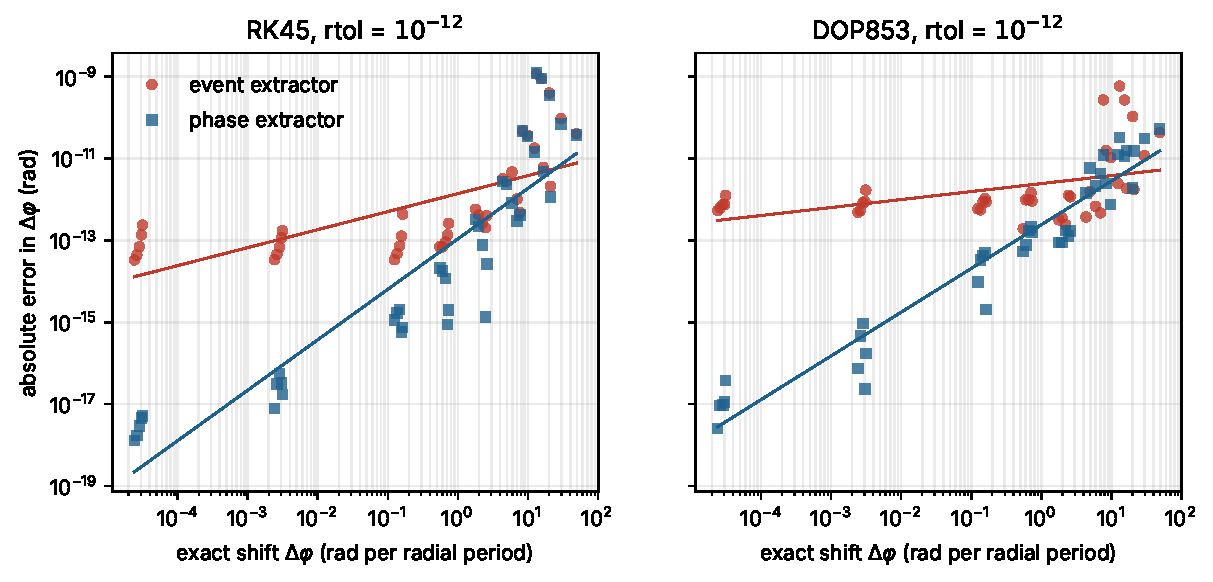
\includegraphics[width=0.9\textwidth]{figures/fig06_error_scaling.pdf}
\caption{End-to-end absolute error against the exact shift at $\mathrm{rtol}=10^{-12}$ with the fits of Table~\ref{tab:fits}.}
\label{fig:scaling}
\end{figure}
\begin{table}[!htbp]
\centering
\caption{Solver comparison on the 40-configuration grid, same-trajectory protocol with $\psi$ in the error control. Median absolute errors in radians.}
\label{tab:solvers}
\begin{tabular}{llcccc}
\toprule
Solver & rtol & phase wins & median ratio & median event err. & median phase err. \\
\midrule
RK45 & $10^{-10}$ & 33 / 40 & 3.03 & $1.5\times10^{-11}$ & $5.2\times10^{-12}$ \\
RK45 & $10^{-12}$ & 35 / 40 & 3.34 & $1.0\times10^{-13}$ & $1.9\times10^{-14}$ \\
DOP853 & $10^{-10}$ & 23 / 40 & 1.64 & $2.2\times10^{-11}$ & $1.2\times10^{-11}$ \\
DOP853 & $10^{-12}$ & 24 / 40 & 1.70 & $3.2\times10^{-13}$ & $1.8\times10^{-13}$ \\
LSODA & $10^{-10}$ & 15 / 40 & 0.92 & $1.0\times10^{-10}$ & $1.9\times10^{-10}$ \\
LSODA & $10^{-12}$ & 18 / 40 & 0.88 & $3.4\times10^{-12}$ & $5.4\times10^{-12}$ \\
Radau & $10^{-10}$ & 32 / 40 & 3.38 & $1.2\times10^{-13}$ & $4.6\times10^{-14}$ \\
Radau & $10^{-12}$ & 34 / 40 & 5.06 & $1.2\times10^{-14}$ & $1.5\times10^{-15}$ \\
\bottomrule
\end{tabular}
\end{table}

\begin{table}[!htbp]
\centering
\caption{Small eccentricity (same-trajectory protocol with $\psi$ in the error control, $\mathrm{rtol}=10^{-12}$, $\rho\in\{10^{-3},0.05,0.5\}$, both solvers): median relative errors.}
\label{tab:smalle}
\begin{tabular}{cccc}
\toprule
$e$ & event & phase & phase wins \\
\midrule
0.0001 & $2.0\times10^{-11}$ & $7.8\times10^{-13}$ & 5 / 6 \\
0.0003 & $6.4\times10^{-12}$ & $4.2\times10^{-13}$ & 5 / 6 \\
0.001 & $4.1\times10^{-12}$ & $4.1\times10^{-14}$ & 5 / 6 \\
0.003 & $8.6\times10^{-13}$ & $1.6\times10^{-14}$ & 5 / 6 \\
0.01 & $7.1\times10^{-13}$ & $2.1\times10^{-14}$ & 5 / 6 \\
0.1 & $1.3\times10^{-12}$ & $2.4\times10^{-14}$ & 5 / 6 \\
\bottomrule
\end{tabular}
\end{table}

\begin{table}[!htbp]
\centering
\caption{Independent check with a 35-digit Taylor-series ODE integration (\texttt{mpmath.odefun}, tolerance $10^{-28}$). Absolute errors of the event and phase estimators against the quadrature reference, and $|w'|$ evaluated at the quadrature's periapsis angle.}
\label{tab:hp}
\small
\begin{tabular}{lcccc}
\toprule
Case & shift (rad) & event err. & phase err. & $|w'(\Phi_{\rm ref})|$ \\
\midrule
Mercury-like & $5.0\times10^{-7}$ & $2.0\times10^{-42}$ & $5.3\times10^{-40}$ & $2.4\times10^{-37}$ \\
e0.3\_rho0.05 & 0.148 & $1.1\times10^{-36}$ & $1.5\times10^{-34}$ & $2.0\times10^{-37}$ \\
e0.3\_rho0.5 & 2.24 & $2.5\times10^{-34}$ & $3.1\times10^{-33}$ & $3.7\times10^{-35}$ \\
e0.3\_rho0.95 & 12.4 & $6.3\times10^{-33}$ & $1.7\times10^{-33}$ & $9.5\times10^{-35}$ \\
e0.9\_rho0.99 & 13.2 & $6.7\times10^{-31}$ & $6.6\times10^{-31}$ & $6.0\times10^{-33}$ \\
e0.001\_rho0.05 & 0.163 & $6.3\times10^{-38}$ & $1.9\times10^{-34}$ & $1.5\times10^{-39}$ \\
cubic\_eps0.01\_e0.3\_g0.003 & 0.229 & $8.8\times10^{-36}$ & $2.2\times10^{-34}$ & $2.5\times10^{-36}$ \\
\bottomrule
\end{tabular}
\end{table}


\begin{thebibliography}{99}\small
\bibitem[Hall(2008)]{Hall2008} K.~A. Hall, ``Exact results for the Kepler problem in general relativity,'' arXiv:0807.4109 [gr-qc] (2008).
\bibitem[Kraniotis(2006)]{Kraniotis2006} G.~V. Kraniotis, ``Periapsis and gravitomagnetic precessions of stellar orbits in Kerr and Kerr--de Sitter black hole spacetimes,'' arXiv:gr-qc/0602056 (2006).
\bibitem[Katsumata et al.(2025)]{Katsumata2025} A.~Katsumata, T.~Harada, K.~Ogasawara and H.~Iizuka, ``New series expansion for the periapsis shift,'' Class. Quantum Grav. \textbf{42}(3), 035004 (2025), doi:10.1088/1361-6382/ada196; arXiv:2408.12977.
\bibitem[Walters(2018)]{Walters2018} S.~J. Walters, ``A simple exact series representation for relativistic perihelion advance,'' Mon. Not. R. Astron. Soc. \textbf{480}(3), 3747--3748 (2018), doi:10.1093/mnras/sty2101.
\bibitem[Della Monica(2025)]{DellaMonica2025} R.~Della Monica, ``PyGRO: A Python integrator for General Relativistic Orbits,'' Astron. Astrophys. \textbf{698}, A193 (2025), doi:10.1051/0004-6361/202554300.
\bibitem[Li et al.(2026)]{Li2026} D.~Li, S.~Hu, C.~Deng, S.~Tan and G.~He, ``Rational orbits and gravitational waves in static spherical spacetimes: an open-source numerical framework,'' arXiv:2606.21029 (2026).
\bibitem[Pantig and \"Ovg\"un(2026)]{PantigOvgun2026} R.~C. Pantig and A.~\"Ovg\"un, ``Phase-plane formulation of weak gravitational deflection in static spherical spacetimes,'' Eur. Phys. J. C \textbf{86}, 1265 (2026), doi:10.1140/epjc/s10052-026-16566-3; arXiv:2608.12423.
\bibitem[Shampine et al.(1991)]{Shampine1991} L.~F. Shampine, I.~Gladwell and R.~W. Brankin, ``Reliable solution of special event location problems for ODEs,'' ACM Trans. Math. Softw. \textbf{17}(1), 11--25 (1991), doi:10.1145/103147.103149.
\bibitem[Shampine and Thompson(2000)]{Shampine2000} L.~F. Shampine and S.~Thompson, ``Event location for ordinary differential equations,'' Comput. Math. Appl. \textbf{39}(5--6), 43--54 (2000), doi:10.1016/S0898-1221(00)00045-6.
\bibitem[Higham(2002)]{Higham2002} N.~J. Higham, \emph{Accuracy and Stability of Numerical Algorithms}, 2nd ed. (SIAM, Philadelphia, 2002).
\bibitem[Dormand and Prince(1980)]{Dormand1980} J.~R. Dormand and P.~J. Prince, ``A family of embedded Runge--Kutta formulae,'' J. Comput. Appl. Math. \textbf{6}(1), 19--26 (1980), doi:10.1016/0771-050X(80)90013-3.
\bibitem[Hairer et al.(1993)]{Hairer1993} E.~Hairer, S.~P. N{\o}rsett and G.~Wanner, \emph{Solving Ordinary Differential Equations I: Nonstiff Problems}, 2nd ed. (Springer, Berlin, 1993).
\bibitem[Virtanen et al.(2020)]{Virtanen2020} P.~Virtanen et al., ``SciPy 1.0: fundamental algorithms for scientific computing in Python,'' Nat. Methods \textbf{17}, 261 (2020).
\bibitem[Montenbruck and Gill(2000)]{Montenbruck2000} O.~Montenbruck and E.~Gill, \emph{Satellite Orbits: Models, Methods and Applications} (Springer, Berlin, 2000).
\bibitem[NASA(2024)]{NASAMercury} NASA Goddard Space Flight Center, ``Mercury Fact Sheet,'' \url{https://nssdc.gsfc.nasa.gov/planetary/factsheet/mercuryfact.html} (accessed November 2026).
\end{thebibliography}

\end{document}
